\section{The inertial measurement unit IMU}
\label{inertial_measurement_unit}

In this section we are going to discuss the Inertial Measurement Unit or IMU. By the end of this section you should be able
to 

\begin{itemize}
\item Describe the operating principles of the two sensors that make up the basic
IMU, an Accelerometer and a Gyroscope. 
\item Model each of these sensors, and account for things like sensor noise and bias. This will be crucial when we incorporate
an IMU into a full-state estimator. 
\end{itemize}



The inertial measurement unit, or IMU measures the movement of
a body in inertial space. Today a certain type of cheap,
mass manufactured IMU, is found in nearly every smartphone,
such as the iPhone X shown in Figure \ref{iphone_x}. 


\begin{figure}[!htb]
\begin{center}
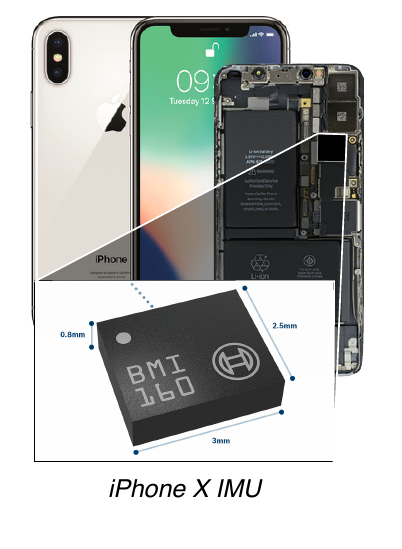
\includegraphics[scale=0.280]{img/hardware/iphone_x.jpeg}
\end{center}
\caption{iPhone X IMU.}
\label{iphone_x}
\end{figure}


Despite their ubiquity today, the development of a sensor that
could accurately track the motion of a moving body was a significant
achievement of the 20th century. The IMU aided transoceanic flights long
before GPS, and was crucial to the Apollo missions as part of the on board guidance,
navigation, and control system. The Apollo spacecraft relied on an IMU
to accurately track both the position, and orientation of the vehicle
on the long voyage to the moon. In space, there are few landmarks
to rely on for guidance. One can track the fixed stars but
this is not easy. The onboard IMU which
operated without the need for such landmarks enabled safe
navigation to the Moon's surface. In modern self-driving cars,
IMUs play a very similar role.  

Generally, an inertial measurement
unit is a composite sensor suite that combines 

\begin{itemize}
\item Three gyroscopes 
\item Three accelerometers 
\end{itemize}

in order to track the exterior
free movement of a rigid body. Some IMUs also incorporate magnetometers,
or a compass, to help track orientation. IMUs come in many shapes and forms. The sensors found in modern
smartphones are relatively cheap, often costing less than a few
dollars when purchased in bulk. They are lightweight and
require relatively little power but produce quite noisy measurements. More expensive IMUs use more complex
components and have more accurate calibration models that can remove the
effects of temperature fluctuations, for example. Let's discuss the components of an IMU. 

\subsection{Gyroscope}

The gyroscope has a long history. The term gyroscope can be quite confusing,
because it refers to several concepts all relating to the idea of measuring
orientation or change in orientation.  Historically, a gyroscope was
a spinning disk that due to its angular momentum resisted
changes in orientation. In the late 19th and early 20th century,
engineers realized that this spinning wheel could be used as
an orientation reference for marine and aeronautical navigations. 

This required precise machining,
and instead of gimbals, it used high quality jewel or
numeric bearings. Although this type of spinning disc
gyroscope can be very accurate, it's quite heavy, bulky and
often very expensive to manufacture. Nevertheless, it is still
using aeronautics and in ballistic applications and
can spin it up to 24000 RPM. 


In a modern gyroscope, the spinning
wheel is typically replaced by a microelectromechanical system that
consists of a small silicon tuning fork that changes its resonance properties
based on an applied rotation or orientation change. These sensors are much cheaper and
can fit in a tiny package. However, they produce
noisy measurements and are sensitive to temperature
based fluctuations. What is more, they measure rotation rates,
and not orientation directly, and so the output signal must be numerically
integrated to determine orientation change. This process can introduce additional
errors into the final orientation estimate.  One would normally think that a spinning
mechanical device would be inferior to a silicon component but
this is not always the case. 


\subsection{Accelerometer}

An accelerometer measures
acceleration along a single axis. Cheaper MEMS based accelerometers
use a miniature cantilever beam with a proof mass attached to it. When the sensor is accelerated,
the beam deflects. This deflection can be measured through
a capacitive circuit for example, and converted into an acceleration value. More expensive sensors may also
use piezoelectric materials. 


\begin{framed}
\theoremstyle{remark}
\begin{remark}{\textbf{Proper Acceleration }}

It's important to note that
an accelerometer measures what's called proper acceleration,
or specific force. 

\begin{equation}
\mathbf{a}_{meas} = \mathbf{f} = \frac{\mathbf{F}_{non-gravity}}{m}
\end{equation}

This is the total non-gravitational
force per unit mass. The proper acceleration is
acceleration with respect to a reference frame in free fall. When you are sitting in your chair,
stationary relative to the ground, the proper acceleration you feel will
be the value of the gravitational acceleration at your location,
but upwards. Another way to say this is that the only
non gravitational force acting on you, the normal force,
must be equal to the force of gravity.
\end{remark}
\end{framed}


However, for
navigational purposes, we often do not care about
our proper acceleration. What we care about is acceleration with
respect to some fixed reference frame. In order to compute this acceleration, we need
to use the fundamental equation for accelerometers in a gravity field. The second derivative opposition,
computed in a fixed frame, is the sum of the specific force,
and the acceleration due to gravity. 

\begin{equation}
\ddot{\mathbf{r}} = \mathbf{f} + \mathbf{g}
\end{equation}

Let's see some examples.

\subsubsection{Example Accelerometer}

An accelerometer in a stationary car measure $\mathbf{g}$ upwards, because the coordinate acceleration is
zero, ignoring the rotation of the Earth. 

\begin{equation}
\mathbf{f} = \ddot{\mathbf{r}} - \mathbf{g} = \mathbf{0} - \mathbf{g}
\end{equation}

Since the force of gravity acts downwards
its negative is the scalar constant $g$ in the upward direction. 


\subsubsection{Example Accelerometer}

Let's look at an example of this on
the International Space Station or ISS. Is the value of $g$ less in low Earth orbit? Well, it is, but only by about 10\% when compared to
the value on the surface of the Earth. The reason why we often hear the term zero-$g$ is because the entire ISS is in free fall together with
the astronauts inside it. An accelerometer rigidly attached to
the station will have a coordinate acceleration equal to $g$. This means that the specific force
measured by an accelerometer will be 0. Another way of saying this is that the
proper acceleration with respect to free fall is zero. The ISS is in free fall. 

In reality residual atmospheric drag and
structural vibrations will create some measured accelerations but they
are typically as low as $10^{-6}g$s. Now, that we know about the basic
principles of gyroscopes and accelerometers, let's discuss
the measurement models we'll need to know in order to
incorporate them into a state estimator. 

\subsection{IMU measurement models}

Let us define an expression for
what a gyroscope measures. The angular rotation rate,
derived from all three gyroscopes, is the angular velocity of the body
frame relative to an inertial frame, expressed in the body frame. 


\begin{equation}
\boldsymbol{\omega}(t) = \boldsymbol{\omega}_s(t) + \mathbf{b}_{gyro}(t) + \mathbf{n}_{gyro}(t)
\end{equation}

where $\boldsymbol{\omega}_s(t)$ is the angular velocity of the sensor expressed in the sensor frame,
$\mathbf{b}_{gyro}(t)$ is the slowly evolving bias and $\mathbf{n}_{gyro}(t)$ is  a white Gaussian additive noise
term to model sensor errors. 

Although gyroscopes do measure the rotation of the Earth, it is often safe to ignore this for applications where we care
only about motion over a short duration. Our accelerometer measurement model
will have similar noise and bias terms but instead of measuring body
accelerations directly as we could do with rotational rates, we need to
explicitly remove the effect of gravity using our fundamental equation for
accelerometers in a gravity field. Since the accelerometers measure
acceleration in the IMU body frame, we will need to keep track of
the orientation at all times in order to be able to perform
the necessary subtraction. 


\begin{equation}
\mathbf{a}(t) = \mathbf{C}_{sn}(t) ( \ddot{\mathbf{r}}_{n}^{sn}(t) - \mathbf{g}_{n}) + \mathbf{b}_{accel}(t) + \mathbf{n}_{accel}(t)
\end{equation}


where $\mathbf{C}_{sn}(t)$ orientation of the sensor (computed by integrating the rotational rates from the gyroscope),
$\mathbf{b}_{accel}(t)$ is a bias term and $\mathbf{n}_{accel}(t)$ is  a noise
term and $\mathbf{g}_{n}$ is the gravity in the navigation frame. 

Let us discuss a few
important limitations of our models. First, an accurate orientation estimate, i.e $\mathbf{C}_{sn}(t)$, is
critical for accurate position estimates. When we convert the measured specific
force into an acceleration we have to make sure that the direction
of gravity is correct. Otherwise, even a small error in
orientation can cause us to think that we are accelerating when we are not. Second, both of the models
we derived ignore the effects of the Earth's rotation. For longer distance navigation,
this is in fact, important. Finally, the models we have
derived are for strapdown IMUs. These are IMUs that are physically
strapped down to the vehicle and do not incorporate
a spinning wheel on gimbals. Although the latter can be much more
accurate, they are rarely used in automotive applications because
of their bulk and their cost. 


\subsection{Summary}

To summarize, in this section we touched upon a 6 degree of freedom IMU and its constituents. Specifically, it is composed of three gyroscopes and
three accelerometers. The gyroscopes measure rotational rates in the sensor frame. Accelerometers measure
the non-gravitational specific force in the sensor frame as well. Since strapdown IMUs are tricky
to calibrate and drift over time, we will need another sensor to periodically
correct our posed estimates. For this, we can use the modern system
of global navigation satellites. 

\subsection{Questions}

\subsection{Assignements}
